\documentclass[conference]{IEEEtran}
\IEEEoverridecommandlockouts
% ---------- Packages ----------
\usepackage[T1]{fontenc}
\usepackage{array}
\usepackage{graphicx}
\usepackage{multirow}
\usepackage{tikz}
\usetikzlibrary{positioning,arrows.meta,fit,backgrounds,calc}
\usepackage{amsmath,amssymb,amsfonts}
% Algorithm packages (template parity; used when the Implementation section is added)
\usepackage{algorithm}
\usepackage{algpseudocode}
\usepackage{textcomp}
\usepackage{xcolor}
\usepackage{booktabs}
\usepackage{soul}
\usepackage{url}
% custom ragged-right paragraph column (defined once, used by all tables)
\newcolumntype{P}[1]{>{\raggedright\arraybackslash}p{#1}}
% NOTE: the template's \usepackage{float} is intentionally omitted here because the
% float package disables captions in double-column table*/figure* environments
% (used for the related-work table and architecture figure). Re-add it with
% \usepackage{dblfloatfix} only if [H] placement is needed later.
% --- spacing helpers (safe for IEEEtran) ---
\usepackage{titlesec}
\titlespacing{\subsection}{0pt}{1.2ex}{0.6ex}
\setlength{\textfloatsep}{6pt plus 2pt minus 2pt}
\setlength{\dbltextfloatsep}{6pt plus 2pt minus 2pt}
\def\BibTeX{{\rm B\kern-.05em{\sc i\kern-.025em b}\kern-.08em
    T\kern-.1667em\lower.7ex\hbox{E}\kern-.125emX}}

\begin{document}
\raggedbottom

% ---------- Title ----------
\title{LLM-Driven Retrieval-Augmented Compliance Auditing for Cloud and Web Privacy}

% ---------- Author ----------
\author{
\IEEEauthorblockN{Aaron Joseph Jean}
\IEEEauthorblockA{
Department of Computer Science\\
University of Galway\\
Galway, Ireland\\
a.jean2@universityofgalway.ie
}
}
\maketitle

% ---------- Abstract ----------
\begin{abstract}
Modern privacy regulations such as the EU General Data Protection Regulation (GDPR), India's Digital Personal Data Protection Act (DPDP), and the California Consumer Privacy Act (CCPA) require organisations to provide clear, accurate disclosures about data collection and to obtain consent before non-essential tracking. Verifying that a website's actual runtime behaviour matches the claims in its written privacy and cookie policies, however, remains a manual, error-prone, and unscalable task. This paper reviews research on automated privacy-compliance assessment across three modalities: natural-language processing of policy text, behaviour-to-policy inconsistency detection, and dynamic web consent auditing, together with the emerging use of large language models (LLMs) for legal reasoning. Rather than separating summary from critique, each research direction is reviewed alongside the specific limitation it leaves unresolved. The review shows that existing systems analyse policy text or runtime behaviour in isolation, while the few hybrid systems are confined to static analysis of compiled mobile binaries. From these observations we derive the central research gap: the absence of a unified, automated framework that ingests runtime web telemetry (HAR logs and JavaScript events), retrieves the relevant legal standard, and cross-references both against scraped policy text using retrieval-augmented generation (RAG) to detect real-world non-compliance. We then describe the design and implementation of such a framework. The pipeline stores regulations in a vector database chunked by article, collects behavioural evidence with an instrumented browser, and asks an LLM to judge each compliance dimension using the retrieved law, the scraped policy and the observed behaviour together. The framework is evaluated on twenty websites across six sectors and four jurisdictions, and every verdict is then checked mechanically against the telemetry it was derived from. The prototype detects contradictions between what a site's policy claims and what the site does, and the verification found no case in which a behavioural claim was fabricated. We also report the failure modes found during testing, the guards added in response, and the limitations that the testing exposed in the pipeline itself.
\end{abstract}

% ---------- Keywords ----------
\begin{IEEEkeywords}
privacy compliance, large language models, retrieval-augmented generation, cookie consent auditing, web telemetry, GDPR, natural language processing
\end{IEEEkeywords}

% =========================
% Section 1: Introduction
% =========================
\section{Introduction}
\subsection{Background}
With the rise of data privacy laws worldwide, including the EU's General Data Protection Regulation (GDPR) and India's Digital Personal Data Protection Act (DPDP), digital transparency has shifted from an ethical preference to a legal mandate. Under these frameworks, organisations are legally required to provide users with clear, detailed, and accurate disclosures regarding data collection, processing purposes, and tracking technologies. Regulations such as the UK's Privacy and Electronic Communications Regulations (PECR) further require explicit user consent before any non-essential tracking technology, such as cookies or device fingerprinting, is initiated. Empirical studies confirm that these requirements are frequently violated in practice: large-scale crawls of consent banners show that many sites set tracking cookies before any user interaction~\cite{trevisan-2019-cookielaw,bouhoula-2024-cookies}, and automated analyses of written policies reveal widespread incompleteness and ambiguity~\cite{wilson-2016-opp115,harkous-2018-polisis}.

\subsection{Motivation}
Despite these legal frameworks, real-world compliance is highly fragmented. Many organisations use template-based privacy policies that do not accurately represent their actual technical practices~\cite{zimmeck-2017-mobileapps}. Conversely, dynamic third-party scripts and marketing pixels are often added to websites without the knowledge of the primary site administrator, leading to silent data leaks and consent violations~\cite{bouhoula-2024-cookies}. Compliance auditing is therefore still performed manually by legal experts and security auditors who inspect website code, examine consent pop-ups, monitor network requests, and read legal documents line by line. This approach is slow, expensive, and unscalable.

While automated tools have been developed to detect trackers or parse privacy policies, they typically operate in silos. Systems either analyse policy text using natural language processing (NLP)~\cite{wilson-2016-opp115,harkous-2018-polisis,ravichander-2019-privacyqa}, or they inspect network traffic to identify tracking scripts and consent violations~\cite{trevisan-2019-cookielaw,bouhoula-2024-cookies}, without cross-referencing the two. The few systems that attempt hybrid auditing are limited to mobile app ecosystems and rely on static program analysis~\cite{zimmeck-2017-mobileapps,zimmeck-2019-maps,xiao-2023-lalaine}, which is prone to false positives from unused libraries and cannot address the runtime complexities of web-based cookie consent banners. In parallel, large language models have begun to demonstrate strong legal-reasoning ability~\cite{guha-2023-legalbench,xie-2025-llmpolicy}, but have not been integrated with live behavioural evidence.

\subsection{Problem Statement}
The main research question addressed by this work is: \textit{How can privacy compliance of web applications be measured in a continuous, contextual, and explainable manner that connects written disclosures (``notice'') to actual software execution (``practice'')?}

\subsection{Paper Organisation}
The remainder of this paper is structured as follows. Section~\ref{sec:litreview} presents an integrated literature review and gap analysis. Section~\ref{sec:approach} derives the framework design from the identified gaps and describes the working implementation, including the scoring algorithm. Section~\ref{sec:results} reports the evaluation: a case study, a batch of twenty sites, the verification of every finding against its telemetry, and the limitations this exposed. Section~\ref{sec:evalplan} sets out the threats to validity and the remaining evaluation, and Section~\ref{sec:conclusion} concludes.

% =========================
% Section 2: Literature Review + Gaps
% =========================
\section{Literature Review and Identified Gaps}
\label{sec:litreview}
To build a sound academic foundation, a systematic search was conducted across IEEE Xplore, the ACM Digital Library, the USENIX proceedings, and Google Scholar, using keyword combinations such as \textit{automated privacy policy compliance}, \textit{cookie consent auditing GDPR}, \textit{deep learning privacy policy NLP}, and \textit{LLM legal compliance evaluation}. Papers were included only if they were published in a reputable peer-reviewed venue (e.g., USENIX Security, IEEE S\&P, NDSS, ACL, EMNLP, NeurIPS, or PoPETs), presented an automated or semi-automated methodology, and collectively spanned both the textual analysis of legal documents and the technical analysis of software behaviour. This yielded ten representative works, organised below into four research directions. Following recent practice, each direction is reviewed together with the specific gap it leaves open, and Table~\ref{tab:related_work} consolidates the comparison.

\subsection{NLP and Machine Learning on Privacy Text}
Analysing unstructured legal text is the first hurdle in automated compliance checking. Wilson et al.~\cite{wilson-2016-opp115} established the foundational benchmark by creating the OPP-115 corpus, manually annotating 115 privacy policies with 23,000 fine-grained data practices and showing that statistical classifiers could automate policy categorisation; however, their models captured only shallow keyword associations rather than deep semantic meaning. Harkous et al.~\cite{harkous-2018-polisis} advanced the field with Polisis, training custom word embeddings on 130,000 policies and using convolutional neural networks to classify policy segments at 88.4\% accuracy, powering an automated question-answering assistant. Ravichander et al.~\cite{ravichander-2019-privacyqa} introduced the PrivacyQA dataset and showed that fine-tuned BERT models could extract answer spans, but reported a large gap between automated models and human legal experts. Crucially, all three rely entirely on the written policy text and have no mechanism to verify whether a site actually follows the stated practices.

\noindent\textit{Gap identified:} Text-only NLP methods assess what a policy \emph{says}, but cannot verify what a system actually \emph{does}~\cite{wilson-2016-opp115,harkous-2018-polisis,ravichander-2019-privacyqa}.

\noindent\textit{Adopted in our framework:} OPP-115's ten data-practice categories~\cite{wilson-2016-opp115} inform the requirement-type taxonomy used to tag legal chunks; Polisis' segment-level classification~\cite{harkous-2018-polisis} motivates routing only topically relevant policy sections to the scorer for long policies, and its finding that domain-specific embeddings outperform general ones supports the choice of legal-domain embeddings; PrivacyQA's demonstration that even legal experts disagree on unanswerable questions~\cite{ravichander-2019-privacyqa} motivates an explicit \textsc{not-addressed} verdict and confidence output rather than forced binary judgements.

\subsection{Behaviour-to-Policy Inconsistency Detection}
A second line of work checks whether disclosures are honest by analysing software behaviour. Zimmeck et al.~\cite{zimmeck-2017-mobileapps} proposed a pioneering hybrid system for Android apps, combining text classification with static analysis of bytecode to detect undisclosed collection of sensitive identifiers. They later scaled this to over one million apps in the MAPS project~\cite{zimmeck-2019-maps}, confirming the scale of violations but remaining specific to compiled Android binaries. Xiao et al.~\cite{xiao-2023-lalaine} shifted the focus to store-mandated privacy labels with Lalaine, characterising widespread non-compliance between Apple privacy labels and observed app behaviour. While these hybrid approaches validate the notice-versus-practice concept, static binary analysis suffers from false positives caused by dead code and, more importantly, cannot capture the dynamic, event-driven behaviour of web applications such as cookie setting and JavaScript-based tracking.

\noindent\textit{Gap identified:} Hybrid notice-versus-practice auditing exists only for mobile ecosystems via static analysis, leaving dynamic web behaviour unaddressed~\cite{zimmeck-2017-mobileapps,zimmeck-2019-maps,xiao-2023-lalaine}.

\noindent\textit{Adopted in our framework:} Zimmeck et al.'s design principle of a closed set of practices checkable in both text and behaviour~\cite{zimmeck-2017-mobileapps} is mirrored in our mapping of each compliance dimension to a defined behavioural evidence type; MAPS' conservative reporting of \emph{potential} non-compliance~\cite{zimmeck-2019-maps} is retained in all generated output; and Lalaine's typology of non-compliance, \emph{neglect}, \emph{contrary}, and \emph{inadequate} disclosure~\cite{xiao-2023-lalaine}, is adopted to classify every policy-versus-telemetry discrepancy the scorer reports.

\subsection{Dynamic Web Cookie and Consent Auditing}
Dynamic auditing of web tracking has been addressed through large-scale crawling. Trevisan et al.~\cite{trevisan-2019-cookielaw} performed a longitudinal study of EU cookie-law compliance, introducing an automated tool that detects tracking cookies set before user consent. Bouhoula et al.~\cite{bouhoula-2024-cookies} extended this to the first general, automated, large-scale analysis of cookie-notice compliance, correcting the selection bias of earlier consent-management-platform-specific studies. Both provide strong empirical evidence of widespread violations, but they focus exclusively on observable network and consent behaviour and do not analyse or cross-reference the text of the websites' written privacy policies.

\noindent\textit{Gap identified:} Dynamic web auditing measures behaviour and consent signals but never reconciles them with the site's written policy claims~\cite{trevisan-2019-cookielaw,bouhoula-2024-cookies}.

\noindent\textit{Adopted in our framework:} Trevisan et al.'s conservative operational definition of a profiling cookie (third-party, present in the intersection of two curated tracker lists, lifetime of at least one month) and their clean-profile, no-interaction visit protocol~\cite{trevisan-2019-cookielaw} are adopted directly by the telemetry collector and HAR evidence extractor; their finding that violations are invariant to client location and browser justifies single-vantage scanning. From Bouhoula et al.~\cite{bouhoula-2024-cookies}, whose crawler and classifiers are open source, we reuse the notice-detection heuristics (filter-list matching combined with z-index inspection), the accept/reject/no-interaction action protocol, and feature-based classification of observed cookie purposes, which removes dependence on tracker blacklists; their conservatively tuned decision-tree mapping from observations to violation types informs our per-dimension verdict rules.

\subsection{LLM-Based Legal and Compliance Evaluation}
The most recent direction applies large language models to legal reasoning. Guha et al.~\cite{guha-2023-legalbench} released LegalBench, a collaboratively built benchmark of 162 legal-reasoning tasks, demonstrating that modern LLMs can interpret legal clauses but evaluating them only on clean, isolated text. Xie et al.~\cite{xie-2025-llmpolicy} took a significant step toward application, systematising 34 privacy-practice clauses from ten modern privacy laws and using an LLM-based pipeline to evaluate policies collected from over 100,000 websites at scale. While this confirms that LLMs can assess policy text against codified law, the evaluation still operates on policy text alone and does not ingest runtime behavioural evidence such as HAR network logs or JavaScript telemetry.

\noindent\textit{Gap identified:} LLMs can reason over legal text and policies, but no framework feeds them live behavioural telemetry to ground their compliance judgements~\cite{guha-2023-legalbench,xie-2025-llmpolicy}.

\noindent\textit{Adopted in our framework:} LegalBench's privacy-related tasks~\cite{guha-2023-legalbench} serve as a pre-deployment benchmark for selecting the scoring LLM, and its IRAC framing (issue, rule, application, conclusion) structures the scoring prompt: the compliance dimension is the issue, the retrieved article the rule, and the policy text plus behavioural evidence the facts to which it is applied. Xie et al.'s systematisation of 34 clauses across ten laws~\cite{xie-2025-llmpolicy} is used to validate the coverage of our compliance dimensions, and their evaluation protocol, measuring per-clause F1 against an expert-annotated sample, is adopted as the evaluation design for the proposed framework.

% ---------- Comparative table (placed at top of page near discussion) ----------
\begin{table*}[!t]
\centering
\caption{Representative Related Work on Automated Privacy-Compliance Auditing}
\label{tab:related_work}
\footnotesize
\begin{tabular}{P{0.9cm} P{2.3cm} P{3.6cm} P{2.0cm} P{2.4cm} P{2.6cm}}
\toprule
\textbf{Ref} & \textbf{Focus} & \textbf{Key Contribution} & \textbf{Modality} & \textbf{Dataset / Evaluation} & \textbf{Limitation} \\
\midrule
\cite{wilson-2016-opp115} & Policy-text corpus & OPP-115 annotated corpus; statistical classification of data practices & Policy text (NLP) & 115 annotated policies & Shallow semantics; no behaviour check \\
\cite{harkous-2018-polisis} & Deep-learning policy analysis & Polisis CNN classifier (88.4\%) and QA assistant & Policy text (NLP) & 130k privacy policies & Text-only; cannot verify site behaviour \\
\cite{ravichander-2019-privacyqa} & Policy QA & PrivacyQA dataset; BERT span extraction & Policy text (NLP) & 1{,}750 questions & Large human--model gap; extractive only \\
\cite{zimmeck-2017-mobileapps} & Notice vs.\ practice (mobile) & Hybrid text + static bytecode analysis & Mobile static & 17{,}991 Android apps & Static; mobile only; false positives \\
\cite{zimmeck-2019-maps} & Compliance at scale & MAPS large-scale automated analysis & Mobile static & 1M+ Android apps & Mobile binaries; no dynamic web consent \\
\cite{xiao-2023-lalaine} & Privacy-label non-compliance & Lalaine measures label vs.\ behaviour gaps & Mobile dynamic/static & iOS apps + label data & iOS labels; not web telemetry \\
\cite{trevisan-2019-cookielaw} & Cookie-law auditing & Detects pre-consent tracking cookies & Web network & Longitudinal EU crawl & Ignores written policy text \\
\cite{bouhoula-2024-cookies} & Cookie-notice compliance & General large-scale consent compliance analysis & Web network/consent & Large-scale web crawl & No policy-text cross-reference \\
\cite{xie-2025-llmpolicy} & LLM policy evaluation & LLM assessment of 34 clauses vs.\ 10 laws & Policy text (LLM) & 100k+ website policies & Policy text only; no runtime telemetry \\
\cite{guha-2023-legalbench} & Legal-reasoning benchmark & LegalBench: 162 legal-reasoning tasks & Legal text (LLM) & 162 tasks, 20 LLMs & Isolated clean text; not applied to web \\
\bottomrule
\end{tabular}
\end{table*}

\subsection{Synthesis and Research Gap}
\label{sec:gap}
Reading across the four directions, the reviewed work collectively establishes three findings: (i) written privacy policies are frequently incomplete and ambiguous and fail to disclose active tracking behaviour~\cite{wilson-2016-opp115,harkous-2018-polisis,ravichander-2019-privacyqa}; (ii) dynamic consent mechanisms on the web frequently set tracking cookies before consent is obtained, constituting measurable GDPR/PECR violations~\cite{trevisan-2019-cookielaw,bouhoula-2024-cookies}; and (iii) large language models can interpret legal clauses and assess policy text against codified law with growing accuracy, but only on text in isolation~\cite{guha-2023-legalbench,xie-2025-llmpolicy}.

Taken together, these findings expose a clear gap. Each strand masters a single modality, policy text, mobile behaviour, web behaviour, or legal reasoning, yet none reconciles the three sources a compliance judgement actually requires. Existing systems analyse the written policy text in isolation (NLP/LLM approaches) or the software and web behaviour in isolation (dynamic crawls), and the few hybrid systems that match policy to behaviour are restricted to static analysis of compiled mobile binaries~\cite{zimmeck-2017-mobileapps,zimmeck-2019-maps,xiao-2023-lalaine}. Consequently, there is currently \textbf{no unified, automated auditing framework that ingests runtime web behavioural evidence (network HAR logs and JavaScript event telemetry), retrieves the relevant legal standards, and cross-references them against scraped policy texts using LLM-driven retrieval-augmented generation (RAG) to detect real-world non-compliance and contradictions}. Bridging this divide between disclosed ``notice'' and observed ``practice'' for the dynamic web is the objective of the framework proposed next.

% =========================
% Section 3: Proposed Approach
% =========================
\section{Framework Design and Implementation}
\label{sec:approach}
The design of the framework is derived directly from the gaps identified in Section~\ref{sec:litreview} rather than chosen in the abstract. Each gap motivates a specific architectural decision, as summarised in Table~\ref{tab:gap_design}. The central observation is that the four research directions each master one modality, policy text, mobile behaviour, web behaviour, or legal reasoning, but none integrates the three sources of evidence that a real compliance judgement requires: the \emph{law} (ground-truth regulation), the \emph{notice} (the site's written policy), and the \emph{practice} (its observed runtime behaviour). The framework is therefore organised around triangulating these three sources for the dynamic web, the setting left unaddressed by prior work. All three phases below are implemented and running; Section~\ref{sec:results} reports first results from live audits.

\begin{table}[!t]
\centering
\caption{Mapping of Identified Gaps to Design Decisions}
\label{tab:gap_design}
\footnotesize
\begin{tabular}{P{0.5cm} P{3.3cm} P{3.4cm}}
\toprule
\textbf{Gap} & \textbf{Limitation in prior work} & \textbf{Design response} \\
\midrule
G1 & Text-only NLP cannot verify behaviour~\cite{wilson-2016-opp115,harkous-2018-polisis,ravichander-2019-privacyqa} & Cross-reference policy claims against runtime telemetry (notice vs.\ practice) \\
\addlinespace
G2 & Hybrid auditing limited to static mobile binaries~\cite{zimmeck-2017-mobileapps,zimmeck-2019-maps,xiao-2023-lalaine} & Dynamic headless-browser instrumentation capturing HAR and JavaScript events \\
\addlinespace
G3 & Web auditing ignores written policy text~\cite{trevisan-2019-cookielaw,bouhoula-2024-cookies} & Couple consent/network evidence with scraped policy extraction per site \\
\addlinespace
G4 & LLMs reason over law but lack grounded evidence~\cite{guha-2023-legalbench,xie-2025-llmpolicy} & RAG over a legal vector store grounds each LLM judgement in retrieved articles \\
\bottomrule
\end{tabular}
\end{table}

\begin{figure*}[!t]
\centering
\resizebox{0.92\textwidth}{!}{%
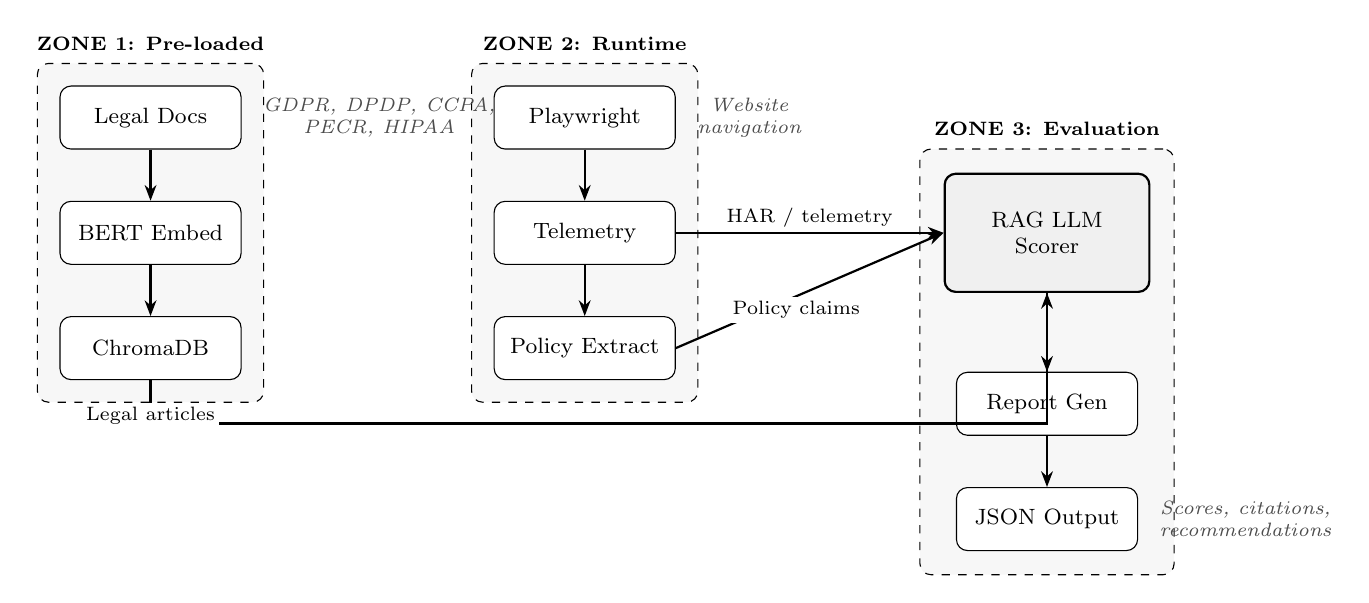
\begin{tikzpicture}[
  font=\footnotesize,
  box/.style={draw, rounded corners, minimum width=2.3cm, minimum height=0.8cm,
              align=center, fill=white},
  scorer/.style={draw, thick, rounded corners, minimum width=2.6cm, minimum height=1.5cm,
              align=center, fill=black!6},
  arr/.style={-{Stealth[length=2mm]}, thick},
  elabel/.style={font=\scriptsize, inner sep=1.5pt, fill=white},
  ilabel/.style={font=\scriptsize\itshape, gray!60!black, align=center}
]
% Zone 1: Pre-loaded (left)
\node[box] (legal) {Legal Docs};
\node[box, below=0.65cm of legal] (bert) {BERT Embed};
\node[box, below=0.65cm of bert] (chroma) {ChromaDB};
\draw[arr] (legal) -- (bert);
\draw[arr] (bert) -- (chroma);
\node[ilabel, right=0.15cm of legal] {GDPR, DPDP, CCPA,\\PECR, HIPAA};
% Zone 2: Runtime (middle)
\node[box, right=3.2cm of legal] (play) {Playwright};
\node[box, below=0.65cm of play] (tele) {Telemetry};
\node[box, below=0.65cm of tele] (policy) {Policy Extract};
\draw[arr] (play) -- (tele);
\draw[arr] (tele) -- (policy);
\node[ilabel, right=0.15cm of play] {Website\\navigation};
% Zone 3: Evaluation (right)
\node[scorer, right=3.4cm of tele] (rag) {RAG LLM\\Scorer};
\node[box, below=1.0cm of rag] (report) {Report Gen};
\node[box, below=0.65cm of report] (json) {JSON Output};
\draw[arr] (rag) -- (report);
\draw[arr] (report) -- (json);
\node[ilabel, right=0.15cm of json] {Scores, citations,\\recommendations};
% Convergence into scorer
\draw[arr] (tele.east) -- node[elabel, above] {HAR / telemetry} (rag.west);
\draw[arr] (policy.east) -- node[elabel, below, pos=0.45] {Policy claims} (rag.west);
\draw[arr] (chroma.south) |- ($(policy.south)+(0,-0.55cm)$)
           node[elabel, below, pos=0.25] {Legal articles} -| (rag.south);
% Zone panels + headers
\begin{scope}[on background layer]
  \node[draw, dashed, rounded corners, fill=black!3, inner sep=0.28cm, fit=(legal)(chroma)] (z1) {};
  \node[draw, dashed, rounded corners, fill=black!3, inner sep=0.28cm, fit=(play)(policy)] (z2) {};
  \node[draw, dashed, rounded corners, fill=black!3, inner sep=0.30cm, fit=(rag)(json)] (z3) {};
\end{scope}
\node[font=\bfseries\scriptsize, above=1pt of z1] {ZONE 1: Pre-loaded};
\node[font=\bfseries\scriptsize, above=1pt of z2] {ZONE 2: Runtime};
\node[font=\bfseries\scriptsize, above=1pt of z3] {ZONE 3: Evaluation};
\end{tikzpicture}}
\caption{Proposed architecture. Three phases converge on a RAG-based LLM scorer: (1) pre-loaded legal ingestion into a vector store, (2) runtime telemetry and policy collection, and (3) compliance evaluation that triangulates retrieved legal articles, HAR/telemetry evidence, and extracted policy claims to produce explainable scores and recommendations.}
\label{fig:architecture}
\end{figure*}

\subsection{Architecture Overview}
The framework consists of three phases (Fig.~\ref{fig:architecture}):
\begin{enumerate}
    \item \textbf{Legal Ingestion (pre-loaded):} Ground-truth regulations (GDPR, DPDP, CCPA, PECR, HIPAA) are parsed and chunked by legal unit (Articles/Sections) to preserve semantic coherence, embedded with a legal-specific model (\textsl{nlpaueb/legal-bert-base-uncased}), and stored in a persistent vector database. This responds to G4: grounding the LLM in retrievable legal text.
    \item \textbf{Runtime Collection:} For a target site, a headless browser (Playwright) simulates navigation, recording outbound requests as an HTTP Archive (HAR) and logging JavaScript/DOM events (consent clicks, canvas fingerprinting). It also crawls and extracts the written Privacy and Cookie policies into structured text. This responds to G2 and G3: capturing dynamic web behaviour and the policy text together.
    \item \textbf{RAG Compliance Evaluation:} For each compliance dimension, the system retrieves relevant legal articles from the vector store, reads the extracted policy claims, parses the behavioural evidence, and prompts an LLM with the combined \emph{law $+$ notice $+$ practice} context to output a score, cite the breached article, and recommend a fix. This responds to G1: verifying practice against stated notice.
\end{enumerate}

\subsection{Design Rationale}
Three decisions follow directly from the literature. First, \textit{legal-specific embeddings} are used because general-purpose models capture only shallow associations on legal text~\cite{wilson-2016-opp115,harkous-2018-polisis}; domain embeddings give terms such as ``controller'' and ``data subject'' appropriate legal semantics, improving retrieval quality. Second, \textit{retrieval-augmented generation} is preferred over prompting an LLM alone because, while LLMs can reason about law~\cite{guha-2023-legalbench,xie-2025-llmpolicy}, ungrounded generation risks hallucinated citations; retrieving the exact article before scoring yields traceable, evidence-backed judgements. Third, \textit{runtime instrumentation} (rather than static analysis) is required because the unaddressed modality is dynamic web behaviour, where consent state changes with user interaction, something static mobile analysis~\cite{zimmeck-2017-mobileapps,zimmeck-2019-maps} cannot observe and text/consent-only studies~\cite{trevisan-2019-cookielaw,bouhoula-2024-cookies} do not reconcile with policy text. Together these choices make the ``notice-to-practice'' verification both possible and explainable, the combination absent from all reviewed work.

\subsection{Implementation Status and Practical Tools}
\label{sec:impl}
The prototype is implemented in Python and organised as independently testable command-line modules, orchestrated end-to-end by a local web frontend:
\begin{itemize}
    \item \textbf{Legal ingestion (complete):} regulations are parsed from official HTML/PDF sources (EUR-Lex, legislation.gov.uk, MeitY) and chunked by legal unit using a multi-statute heading grammar (\textsl{Article~7} for GDPR/DPDP, \textsl{6.---(1)} UK-SI numbering for PECR, \textsl{1798.100.}\ for the CCPA); heading-only fragments are discarded. GDPR yields exactly 99 article chunks. Chunks carry regulation, article, requirement-type and severity metadata and are embedded into a persistent ChromaDB collection.
    \item \textbf{Runtime collection (complete):} a Playwright-instrumented Chromium visit records the HAR, hooks fingerprinting APIs (canvas, WebGL, AudioContext, WebRTC, battery, fonts) via an injected trap script, tags consent-related UI elements, and extracts policy links; a separate scraper exports the site's privacy and cookie policies as markdown. The evidence extractor applies the conservative profiling-cookie rule of~\cite{trevisan-2019-cookielaw} (third-party $\wedge$ present in the intersection of two tracker lists $\wedge$ lifetime $\geq$ 30 days) and also recovers JavaScript-set cookies from browser context state, which header-only analysis misses.
    \item \textbf{RAG evaluation (complete):} per dimension, the scorer retrieves law chunks (metadata-filtered semantic search plus deterministic \emph{dimension-anchored} fetches of the dimension's known articles), injects the full policy text and the selected behavioural evidence, and prompts an LLM (temperature 0, strict JSON) for a verdict. The scorer is provider-agnostic (OpenAI and Anthropic backends).
    \item \textbf{Reporting (complete):} verdicts are aggregated severity-weighted and rendered as a self-contained HTML report; a local web frontend runs the full pipeline per URL with a live stage log.
\end{itemize}
During implementation the embedding model had to be changed. Legal-domain BERT (\textsl{nlpaueb/legal-bert-base-uncased}) was chosen initially for its legal vocabulary, but retrieval tests showed near-uniform cosine similarities (about 0.72 for every chunk) and effectively random ranking. It is a raw masked-language model without sentence-level training, so the vocabulary advantage did not help retrieval. It was replaced with a sentence-trained encoder (\textsl{all-mpnet-base-v2}), after which the expected articles ranked first.

\subsection{Scoring Strategy}
For each dimension the LLM returns a structured judgement rather than a bare score. It contains: a \textbf{score} (0--100, anchored to a rubric), a \textbf{verdict} (\textsc{pass}, \textsc{fail}, \textsc{partial}, or \textsc{not-addressed}) with a \textbf{confidence} value, following the abstention lesson of~\cite{ravichander-2019-privacyqa}; the \textbf{breached article}, quoted from the retrieved text only; the \textbf{policy claim} quoted from the notice; the \textbf{behavioural evidence} relied upon; a \textbf{discrepancy type} (\emph{neglect} / \emph{contrary} / \emph{inadequate}, the typology of~\cite{xiao-2023-lalaine}); and a plain-English explanation and recommended fix. Dimension scores are aggregated using severity weights (critical 3, high 2, medium 1, low 0.5), with \textsc{not-addressed} dimensions excluded; all output is framed as \emph{potential} non-compliance~\cite{zimmeck-2019-maps}.

\begin{algorithm}[!t]
\caption{Per-dimension RAG compliance scoring}
\label{alg:scoring}
\begin{algorithmic}[1]
\Require target site $s$; dimensions $D$; regulations $R$; vector store $V$
\Ensure severity-weighted report with article-cited verdicts
\State $H \leftarrow$ \textsc{CollectTelemetry}($s$) \Comment{HAR, JS alarms, consent UI}
\If{$H$ is degenerate (bot-blocked / empty capture)}
    \State \textbf{return} \textsc{InsufficientData} \Comment{refuse to score garbage input}
\EndIf
\State $E \leftarrow$ \textsc{ExtractEvidence}($H$) \Comment{profiling-cookie rule~\cite{trevisan-2019-cookielaw}}
\State $P \leftarrow$ \textsc{ScrapePolicies}($s$)
\For{each dimension $d \in D$}
    \State $e_d \leftarrow$ evidence in $E$ matching $d$'s evidence keys
    \If{$P = \emptyset$ \textbf{and} $e_d = \emptyset$}
        \State verdict $\leftarrow$ \textsc{not-addressed} \Comment{deterministic guard; no LLM call}
    \Else
        \State $L_d \leftarrow$ anchored articles($d$) $\cup$ filtered search($V, d, R$)
        \State verdict $\leftarrow$ \textsc{LLM}$_{T=0}$(IRAC: issue $d$, rule $L_d$, facts $P + e_d$)
        \State validate JSON; clamp score/confidence; check verdict enum
    \EndIf
\EndFor
\State \textbf{return} severity-weighted aggregate + per-dimension verdicts
\end{algorithmic}
\end{algorithm}

The full scoring procedure, including the two deterministic guards added after the error analysis of Section~\ref{sec:results}, is given in Algorithm~\ref{alg:scoring}.

\subsection{Techniques and Artifacts Adopted from Reviewed Work}
\label{sec:adopted}
Beyond motivating the gap, the reviewed papers contribute reusable techniques, datasets, and open-source artifacts that are incorporated into the implementation. Table~\ref{tab:adopted} consolidates this mapping from source to framework component. Publicly released artifacts are reused where licences permit: the crawler and classifiers of~\cite{bouhoula-2024-cookies}, the measurement tool and dataset of~\cite{trevisan-2019-cookielaw}, the OPP-115 corpus~\cite{wilson-2016-opp115}, the PrivacyQA dataset~\cite{ravichander-2019-privacyqa}, and the LegalBench task suite~\cite{guha-2023-legalbench}.

\begin{table}[!t]
\centering
\caption{Elements Adopted from Reviewed Work into the Proposed Framework}
\label{tab:adopted}
\footnotesize
\begin{tabular}{P{0.5cm} P{3.6cm} P{3.1cm}}
\toprule
\textbf{Ref} & \textbf{Adopted element} & \textbf{Framework component} \\
\midrule
\cite{trevisan-2019-cookielaw} & Conservative profiling-cookie rule (dual tracker-list intersection, $\geq$1-month lifetime); clean-profile no-interaction visits & HAR evidence extractor; telemetry collection protocol \\
\addlinespace
\cite{bouhoula-2024-cookies} & Notice-detection heuristics; accept/reject action protocol; feature-based cookie-purpose classification & Consent-interaction module; violation decision rules \\
\addlinespace
\cite{wilson-2016-opp115} & Ten data-practice categories; annotated corpus & Legal-chunk metadata taxonomy; evaluation data \\
\addlinespace
\cite{harkous-2018-polisis} & Segment-level policy classification; domain-specific embeddings & Section routing for long policies; embedding choice \\
\addlinespace
\cite{ravichander-2019-privacyqa} & Unanswerability of some policy questions & \textsc{not-addressed} verdict; confidence output \\
\addlinespace
\cite{zimmeck-2017-mobileapps} & Closed set of practices checkable in text and behaviour & Dimension-to-evidence-type mapping \\
\addlinespace
\cite{zimmeck-2019-maps} & Tiered analysis for scale; ``potential'' non-compliance phrasing & Two-tier LLM usage; report language \\
\addlinespace
\cite{xiao-2023-lalaine} & Neglect / contrary / inadequate disclosure typology & Discrepancy classification in scorer output \\
\addlinespace
\cite{guha-2023-legalbench} & Privacy-task benchmark; IRAC prompt framing & Scorer-LLM selection; scoring prompt structure \\
\addlinespace
\cite{xie-2025-llmpolicy} & 34-clause systematisation over ten laws; expert-annotated F1 protocol & Dimension coverage validation; evaluation design \\
\bottomrule
\end{tabular}
\end{table}

% =========================
% Section 4: Preliminary Results
% =========================
\section{Evaluation}
\label{sec:results}
The framework was evaluated in three stages. A single site was audited in detail to establish that the pipeline produces usable findings, a batch of twenty sites was then audited to measure coverage and behaviour across sectors, and every verdict in that batch was checked mechanically against the telemetry it was derived from. The third stage exists because an LLM-based auditor is only useful if its findings can be shown to come from the evidence rather than from the model. All figures below are from the run of 16 August 2026 using gpt-4o-mini at temperature 0.

\subsection{Case Study: Live Audit of a News Website}
The prototype's first end-to-end audit targeted \textsl{www.independent.ie} (news media --- the category with the highest violation rates in~\cite{trevisan-2019-cookielaw}), scored against GDPR and PECR with a clean-profile, no-interaction visit. The telemetry recorded \textbf{22 third-party domains} contacted before any consent, including \textbf{15 tracker eTLD+1s} (among them doubleclick.net, taboola.com and google-analytics.com), \textbf{4 fingerprinting API calls} (WebRTC $\times$3, Battery API), and \textbf{zero pre-consent profiling cookies} under the strict detection rule. Table~\ref{tab:results} summarises the verdicts.

\begin{table}[!t]
\centering
\caption{Audit verdicts for www.independent.ie (GDPR + PECR)}
\label{tab:results}
\footnotesize
\begin{tabular}{P{2.6cm} P{1.4cm} P{3.2cm}}
\toprule
\textbf{Dimension} & \textbf{Verdict} & \textbf{Key finding} \\
\midrule
Tracking without consent & \textsc{fail} (18) & tracker requests + fingerprinting before any consent; discrepancy: \emph{contrary} \\
\addlinespace
Disclosure of third parties & \textsc{fail} & no recipients named in policy; 15 tracker domains observed \\
\addlinespace
Pre-consent tracking cookies & \textsc{partial} (50) & no profiling cookies observed; consent UI present \\
\bottomrule
\end{tabular}
\end{table}

This case shows why the three sources need to be combined. The site's consent platform does withhold cookies, so a cookie-only audit in the style of~\cite{trevisan-2019-cookielaw} would find little. However, tracker requests and fingerprinting calls still run before consent, and the written policy does not name any of the observed recipients. The contradiction only becomes visible when the law, the notice and the behaviour are examined together.

\subsection{Batch Evaluation Across Twenty Websites}
\label{sec:batch}
To test the pipeline beyond a single case, twenty sites were selected across six sectors and four jurisdictions. The selection deliberately includes sectors at both ends of the range reported by Trevisan et al.~\cite{trevisan-2019-cookielaw}, namely news media and government, and two sites known to use bot protection so that the failure path would also be exercised. Each site was audited on three dimensions (pre-consent tracking, tracking without consent, disclosure of third parties) against GDPR and PECR, with DPDP added automatically for Indian domains. The harness records the outcome of every stage, so sites that fail are counted rather than silently dropped.

\begin{table}[!t]
\centering
\caption{Coverage outcomes over twenty sites}
\label{tab:coverage}
\footnotesize
\begin{tabular}{P{3.4cm} c P{3.2cm}}
\toprule
\textbf{Outcome} & \textbf{Sites} & \textbf{Cause} \\
\midrule
Scored & 15 & --- \\
Capture refused & 2 & bot protection; degenerate capture rejected by the sanity gate \\
\addlinespace
Collection timed out & 2 & slow sites exceeding the collector budget \\
\addlinespace
Insufficient data & 1 & no policy retrieved and no relevant events observed \\
\bottomrule
\end{tabular}
\end{table}

Table~\ref{tab:coverage} gives the coverage outcome. Fifteen of twenty sites produced a scored report. Two sites (irctc.co.in and ndtv.com) were refused by the capture sanity gate, which is the intended behaviour: both returned effectively empty pages under a headless browser, and scoring such a capture would produce confident findings about nothing. A further two sites exceeded the collection timeout, and one site produced a report of \textsc{insufficient-data} because neither a policy nor relevant behavioural events could be obtained. The overall capture failure rate is therefore 10\%, and the rate at which the pipeline declines to give a compliance opinion is 25\%.

\begin{table}[!t]
\centering
\caption{Mean score by sector (higher is more compliant)}
\label{tab:sector}
\footnotesize
\begin{tabular}{P{2.3cm} c c P{2.3cm}}
\toprule
\textbf{Sector} & \textbf{Sites} & \textbf{Mean} & \textbf{FAIL verdicts} \\
\midrule
Government & 1 & 53.0 & 0 / 3 \\
SaaS & 1 & 44.0 & 0 / 3 \\
Education & 4 & 29.2 & 7 / 12 \\
News & 6 & 24.3 & 8 / 18 \\
Social & 1 & 25.0 & 1 / 3 \\
E-commerce & 2 & 3.0 & 4 / 6 \\
\bottomrule
\end{tabular}
\end{table}

Table~\ref{tab:sector} reports the mean score by sector. The ordering is broadly consistent with the published sector pattern: the government site scores highest and news media sits in the lower half. The result should not be over-read. Several sectors are represented by a single site, and the e-commerce mean is depressed by the confound discussed in Section~\ref{sec:limits}. Across all scored sites the mean was 26.1 and the range 0 to 53, but only seven distinct scores occurred in fifteen reports. The model anchors on the round values of the scoring rubric rather than using the full scale, so the scores are better treated as an ordinal ranking than as interval measurements.

At the level of individual dimensions, tracking without consent produced ten \textsc{fail} verdicts, four \textsc{partial} and one \textsc{pass}, and disclosure of third parties produced seven \textsc{fail} and eight \textsc{partial}. Pre-consent tracking produced only three \textsc{fail} verdicts and ten \textsc{partial}, because the strict profiling-cookie rule rarely fires on sites that operate a consent platform. That dimension therefore carries less discriminating information than the other two, which is a useful finding in itself: the cookie-based test that the earlier literature relies on is the weakest of the three signals on the current web, while request-level and disclosure-level evidence separate sites much more clearly.

\subsection{Verifying Findings Against the Telemetry}
\label{sec:verify}
Compliance findings produced by a language model are only credible if each claim can be traced to the artefact it came from. A verification tool was therefore written that re-checks every verdict mechanically, without invoking a model, so that the check itself cannot fabricate. To make this possible the scorer records, for every verdict, which legal articles were retrieved and the exact rule text that was placed in the prompt.

Five checks are applied to each verdict. The first confirms that the cited article was actually retrieved for that dimension. The second confirms that the quoted legal requirement appears in the retrieved rule text. The third confirms that the quoted policy claim appears in the scraped policy. The fourth confirms that every domain, cookie name and count named in the finding exists in the evidence extracted from the HAR file. The fifth applies internal consistency rules, for example that a \textsc{not-addressed} verdict carries no breach citation and that a discrepancy type is asserted only when both a policy quotation and behavioural evidence are present. Quotation matching normalises whitespace and quotation marks and accepts elided quotations, but reports anything below a high similarity threshold as a paraphrase rather than a quotation.

\begin{table}[!t]
\centering
\caption{Attribution of the five flagged claims}
\label{tab:flags}
\footnotesize
\begin{tabular}{P{2.9cm} c P{3.5cm}}
\toprule
\textbf{Cause} & \textbf{Flags} & \textbf{Interpretation} \\
\midrule
Over-claim on missing input & 4 & non-disclosure asserted about a policy that was never retrieved \\
\addlinespace
Unlocatable quotation & 1 & quoted requirement not located in the retrieved article text \\
\midrule
Fabricated behavioural claim & 0 & no invented domain, cookie or count \\
\bottomrule
\end{tabular}
\end{table}

Across the fifteen scored reports the verification flagged five claims, and the mean grounding rate, that is, the proportion of dimensions in which every claim could be traced to its source, was 86.7\%. Each flag was inspected individually and the attribution is given in Table~\ref{tab:flags}. Four occurred on sites where no policy document could be retrieved, and in every case the model had asserted a discrepancy type of \emph{neglect}, that is, that a practice had not been disclosed in a document it had never been shown. Non-disclosure cannot be established from an unread policy, so this is genuine over-claiming; it is now rejected by the consistency rules and constrained in the prompt. The remaining flag is a paraphrase of a definition of consent that appears in GDPR Article 4(11) rather than in the retrieved Article 7 text, so the statement is legally accurate but is not a quotation of the rule that was supplied.

Two defects were also found in the verification tool itself during this analysis and corrected: names of fingerprinting APIs such as \texttt{navigator.getBattery} matched the pattern used to detect domain names, and elided quotations were tested after their ellipsis markers had been removed, so valid quotations spanning a gap were reported as unmatched. Both inflated the apparent error rate of the model. This is worth recording because it illustrates a general difficulty in evaluating a generative system: the measuring instrument requires validation of its own.

The result that matters for the reliability of the approach is the last row of Table~\ref{tab:flags}. No claim was found in which the model asserted a behavioural event that did not appear in the telemetry. Every domain, cookie and fingerprinting call named in the fifteen reports was present in the corresponding HAR evidence. The errors that did occur were of two kinds: quoting loosely, and reasoning about a document that had not been retrieved. Both are addressable by constraining the prompt, and both are detectable without human review, which is what makes the check usable at scale.

\subsection{Limitations Revealed by Testing}
\label{sec:limits}
The batch exposed three limitations that were not visible from a single case study.

\emph{Policy retrieval dominates the score.} Sites for which no policy document was retrieved scored 0.0 on average, while sites with one or two policy documents scored 32.6. A gap of roughly thirty-three points is attributable to the auditing pipeline's own retrieval coverage rather than to the behaviour of the site. Two causes were identified: policies hosted on a parent company domain, which the same-domain preference of the scraper misses, and pages that render policy links only after JavaScript execution. Results for sites without a retrieved policy must therefore be reported separately, and are excluded from the sector means where noted.

\emph{Bot protection bounds the achievable coverage.} Two sites could not be captured at all and two more exceeded the collection budget. Because the sanity gate refuses to score a degenerate capture, this manifests as reduced coverage rather than as wrong answers, which is the preferable failure mode, but it does mean that the sites most likely to engage in aggressive tracking are also among the hardest to audit.

\emph{Jurisdiction determines the applicable instrument.} The ePrivacy Directive is transposed nationally, so the cookie-consent rule differs by country even though the GDPR applies uniformly across the Union. An early version of the batch scored every site against the GDPR and the UK Privacy and Electronic Communications Regulations, which is incorrect for the eleven Irish sites in the sample: Ireland transposed the Directive through S.I. 336/2011, whose Regulation 5(3) is the operative provision and is enforced by the Data Protection Commission. The framework now selects instruments by jurisdiction, and the Irish instrument has been ingested alongside the others; the results reported in this section, however, predate that correction, so the ePrivacy citations for Irish sites in this run name the UK instrument. The GDPR findings, which account for the disclosure dimension, are unaffected, and re-scoring the Irish sample under S.I. 336/2011 is immediate remaining work. The episode is worth recording because it is a failure mode that a single-jurisdiction evaluation would never expose, and because cross-border auditing tools that assume one ePrivacy text are subject to it.

A related observation supports the retrieval-based design. The corpus holds consolidated legislation, so the ingested PECR text includes the substitution of Regulation 6 and the insertion of Schedule A1 by the Data (Use and Access) Act 2025, in force from February 2026, which moves statistical cookies from an opt-in to an opt-out basis under defined conditions. The system therefore reasons over the amended rule without any change to the model, because the law is held in the vector store rather than in model weights. A system that had internalised the earlier rule during training would continue to apply it.

\emph{Score granularity is coarse.} With seven distinct values across fifteen sites, the numeric score should not be treated as a continuous measurement. The verdict labels and the underlying evidence carry the information; the score is best used to rank sites rather than to quantify the distance between them.
Testing surfaced three failure modes, each fixed at the layer that caused it and re-verified:
\begin{enumerate}
    \item \textbf{LLM over-condemnation.} In an early run the pre-consent-tracking dimension returned \textsc{fail} (score 0, confidence 1.0) although no profiling cookies had been observed: the model invented cookie installations and misread the audit protocol line (``consent interaction: none'') as the \emph{site} lacking a consent mechanism. \emph{Fix:} evidence-discipline rules in the system prompt (cite only listed events; empty evidence forbids behavioural violations) and an explicit audit-protocol note in the evidence block. On re-run the verdict flipped to \textsc{partial} with policy-only reasoning and \texttt{behavioral\_evidence: null}.
    \item \textbf{Retrieval near-miss.} One verdict cited GDPR Art~19 (rectification notification) instead of Art~13(1)(e) (disclosure of recipients). Semantic similarity had ranked the wrong ``recipients'' article first, and the model correctly obeyed the instruction to cite only retrieved text. \emph{Fix:} dimension-anchored retrieval (Section~\ref{sec:impl}). This also supports the grounding design: the failure moved from the generation step to the retrieval step, where it could be fixed deterministically.
    \item \textbf{Degenerate capture.} A bot-blocked site (\textsl{www.ndtv.com}) produced an empty capture (1 request, 0 UI elements), and the scorer initially issued confident \textsc{fail} verdicts on nothing, treating the unretrieved policy as proof that none exists. \emph{Fix:} a capture sanity gate that refuses to score degenerate scans, and an insufficiency guard: with no policy text and no behavioural events the verdict is forced to \textsc{not-addressed} without invoking the LLM, and the overall verdict becomes \textsc{insufficient-data}.
\end{enumerate}
Together with the embedder change in Section~\ref{sec:impl}, these are four documented findings from the implementation phase. A fifth was added by the batch: on sites where the policy could not be retrieved, the model inferred non-disclosure from the absence of a document rather than abstaining, which is now prevented.

% =========================
% Section 5: Evaluation Plan
% =========================
\section{Threats to Validity and Remaining Evaluation}
\label{sec:evalplan}
Three threats to validity follow from the design of the study. The ground truth for compliance is not established independently: the batch measures what the system reports and whether those reports are grounded in the evidence, but not whether a lawyer would agree with the verdicts. Establishing that requires hand annotation, which is the principal item of remaining evaluation and follows the per-clause protocol of~\cite{xie-2025-llmpolicy}: a sample of sites annotated against the article text, from which per-dimension precision, recall and F1 are computed. A single annotator is a known weakness, acknowledged in the light of the expert disagreement reported by~\cite{ravichander-2019-privacyqa}.

The second threat is sample size. Six sectors across fifteen scored sites is sufficient to expose pipeline limitations, but not to make claims about sector-level compliance rates; several sectors are represented by a single site.

The third threat is that a single model was used throughout. Model selection has not yet been made empirically, and the intended comparison uses the LegalBench privacy tasks~\cite{guha-2023-legalbench} together with the annotated sample. Reproducibility is supported by temperature-0 scoring, pinned tracker lists and versioned prompts; repeat-run variance is to be reported alongside the F1 results.

% =========================
% Section 6: Conclusion
% =========================
\section{Conclusion and Future Work}
\label{sec:conclusion}
This paper reviewed automated privacy-compliance research across four directions and showed that no prior system integrates the three evidence sources a compliance judgement requires: the law, the site's written notice, and its observed runtime practice. We then presented the design and implementation of a framework that closes this gap for the dynamic web. Regulations are chunked by legal unit into a vector store, behavioural evidence is captured with an instrumented browser, and an LLM scores each compliance dimension using the retrieved law, the scraped policy and the observed behaviour under an IRAC structure. In live audits the prototype detected a site whose trackers and fingerprinting run before consent while its policy names no recipients, which no single-modality system could have shown. A batch of twenty sites produced fifteen scored reports, with the remainder declined rather than guessed at. Mechanical verification of every verdict against its own telemetry gave a grounding rate of 86.7\% and found no case in which the model asserted a behavioural event that the evidence did not contain; the errors that did occur were reasoning about policies that had not been retrieved, and one paraphrase of a definition drawn from an article that had not been supplied. Both are correctable in the prompt and both are detectable without human review. Testing also showed that the pipeline's own retrieval coverage, rather than site behaviour, accounts for roughly thirty-three points of score difference where policies could not be obtained, which is the most significant limitation of the current system. Future work includes consent-banner interaction with accept/reject differential testing, following~\cite{bouhoula-2024-cookies}; the evaluation plan of Section~\ref{sec:evalplan}; and post-login observation, i.e.\ comparing what a site collects inside an authenticated session with the consent that was given, which none of the reviewed papers address.

% =========================
% Section 7: Use of AI
% =========================
\section{Use of AI}
\label{sec:ai}
In line with the capstone guidelines, the use of AI tools is declared. AI assistance (large language model tools) was used during this project as a coding and writing aid: for LaTeX formatting and structuring of this document, for drafting and revising sections of the text, and for assistance during the implementation and debugging of the prototype. The research direction, design decisions and experiments are the author's own.

% =========================
% Acknowledgment
% =========================
\section*{Acknowledgment}
The author thanks Dr.\ Ihsan for his supervision throughout this capstone project, and in particular for the critique at the interim review that led to the multi-site evaluation and the verification of findings against the collected telemetry reported in Section~\ref{sec:results}. The author also acknowledges the maintainers of the Disconnect and Ghostery tracker databases, and the Irish Statute Book, EUR-Lex and legislation.gov.uk services, whose openly published texts made the legal corpus possible.

% ---------- Bibliography ----------
\bibliographystyle{ieeetr}
\bibliography{reference}

\end{document}
